\documentclass[a4paper]{article}

\usepackage[swedish]{babel}
\usepackage[utf8x]{inputenc}
\usepackage{amsmath}
\usepackage{amssymb}
\usepackage[T1]{fontenc}
\usepackage{graphicx}
\usepackage{epstopdf}

\begin{document}

\section*{1.1}

Enligt uppgiften skall

\begin{equation*}
	v(x,y) = x^3 + axy^2 - 3x^2y + y^3
\end{equation*}

bestämmas som imaginärdelen av en holomorf funktion $f(z) = f(x + iy) = u + iv$. Eftersom $f$ skall vara holomorf så kommer $u$ och $v$ att vara harmoniska (enl. sats 3.22\cite{boken},) vilket medför att $\nabla^2v = v''_{xx} + v''_{yy} = 0$, där derivatorna ges av

\begin{align*}
	&\begin{cases}
		v'_x = 3x^2 + ay^2 - 6xy\\
		v'_y = 2axy - 3x^2 + 3y^2\\
	\end{cases}
	,\quad
	\begin{cases}
		v''_{xx} = 6x - 6y\\
		v''_{yy} = 2ax + 6y\\
	\end{cases}\\
	&\\
	&\nabla^2v = v''_{xx} + v''_{yy} = 0\\
	&\iff 6x - 6y + 2ax + 6y = 0\\
	&\iff x(6+2a) = 0\\
	&\implies a = -3.
\end{align*}

Till följd av Cauchy Riemanns ekvationer kan derivatan av $f$ skrivas som 

\begin{align*}
	f'(x + iy)	&= u'_x(x,y) + iv'_x(x,y) = v'_y(x,y) + iv'_x(x,y)\\
				&= (3x^2 - 3y^2 - 6xy) + i(-6xy - 3x^2 + 3y^2).\\
\end{align*}

Om sedan $x,y$ sätts till $x = z, y = 0$ respektive så kan derivatan skrivas som ett uttryck i enbart z

\begin{align*}
	f'(z) = 3z^2 - i3z^2
	\implies f(z) = \int f'(z)dz = z^3 - iz^3 + C.
\end{align*}

Begynnelsevilkoret $f(0) = 1$ ger sedan att $C = 1$. $f$ blir då

\begin{equation*}
	f(z) = z^3 - iz^3 + 1.
\end{equation*}

\section*{1.2}

Med hjälp av Eulers formel för sinusfunktionen kan uppgiften skrivas enligt

\begin{align*}
	&\sin z	= 2i \iff \frac{e^{iz} - e^{-iz}}{2i} = 2i\\
	&\iff e^{iz} - e^{-iz} = -4.
\end{align*}

Utför variabelbytet $w = e^{iz}$

\begin{align*}
	&e^{iz} - e^{-iz} = -4 \iff w^2 - 1 + 4w = 0\\
	&\implies	\begin{cases}
					w_1 = -2 + \sqrt{5}\\
					w_1 = -2 - \sqrt{5}
				\end{cases}.
\end{align*}

Sedan fås $z_1$ från det tidigare variabelbytet

\begin{align*}
	w_1 &= e^{iz_1} \implies iz_1 = \text{Log}(-2 + \sqrt{5})\\
		&= \ln|-2 + \sqrt{5}| + i\text{Arg}(-2 + \sqrt{5})\\
		&= \ln(2+\sqrt{5}) + i(0 + 2\pi k), k \in \mathbb{Z}\\
	 &\implies z_1 = 2\pi k - i\ln(2+\sqrt{5}), k \in \mathbb{Z}.
\end{align*}

Här används principalgrenen av den komplexa logaritmen eftersom $w_1$ ligger på den positivia reella axeln. Samma räkningar kan utföras för att få fram $z_2$, dock används istället den naturliga grenen av logaritmen då $w_2$ ligger på den negativa reella axeln.

\begin{align*}
	w_2 &= e^{iz_2} \implies iz_2 = \log(-2 - \sqrt{5})\\
		&= \ln(2+\sqrt{5}) + i\text{arg}(-2 - \sqrt{5})\\
	 &\implies z_2 = \pi + 2\pi k - i\ln(2 + \sqrt{5}), k \in \mathbb{Z}.
\end{align*}

\section*{1.3}
\subsection*{a)}

\begin{figure}[h!]
	\centering
	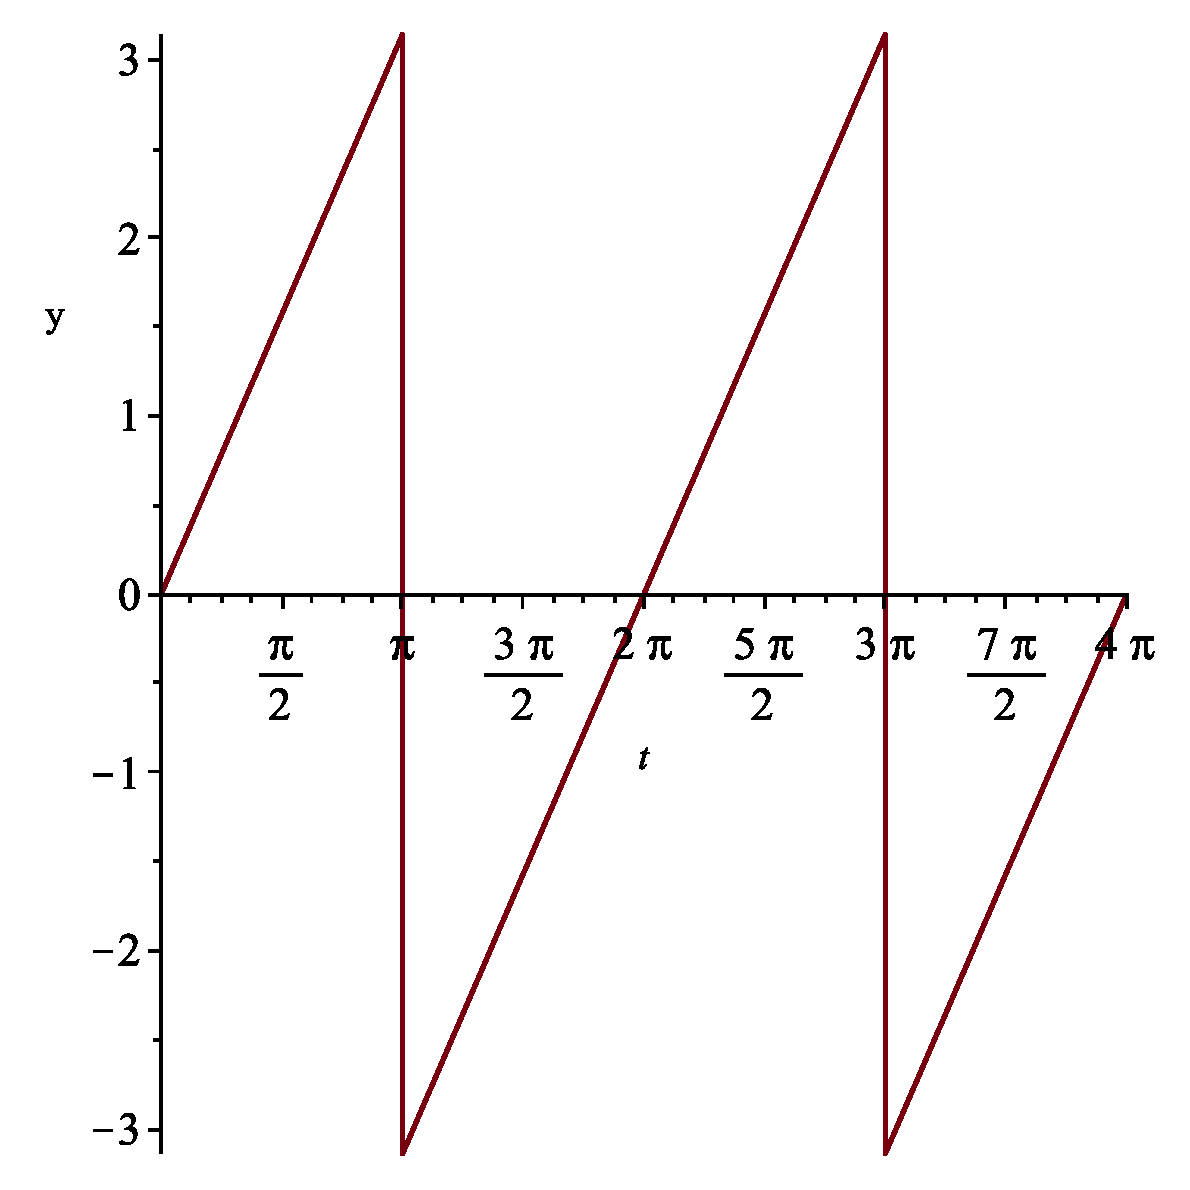
\includegraphics[width=0.5\textwidth]{plot1_2.eps}
	\caption{Plot av $y = \text{Im}(\text{Log}(e^{it})), 0 \leq t \leq 4\pi$ där Log är principalgrenen av logaritmen.}
	\label{fig:1_2}
\end{figure}

I Figur \ref{fig:1_2} ses det att $y = \text{Im}(\text{Log}(e^{it}))$ är $2\pi$-periodisk. Detta för att principalgrenen av logaritmen $\text{Log}(z)$ bara är definierad för $-\pi (+2\pi k)< \text{Arg}(z) < \pi (+2\pi k), k \in \mathbb{Z}$. Definitionen av den komplexa logaritmen ger

\begin{align*}
	\text{Log}(e^{it})	&= \ln|e^{it}| + i\text{Arg}(e^{it})\\
						&= \ln|e^{it}| + it\\
						&= it, -\pi < t < \pi (+2\pi k).
\end{align*}

Funktionen $y = \text{Im}(\text{Log}(e^{it}))$ blir då linjär $y = Im(it) = t)$ för $-\pi < t < \pi (+2\pi k)$, vilket motsvarar de linjära streckorna i Figur \ref{fig:1_2}. Därutöver är inte funktionen definierad då $t$ är en mulitpel av $2\pi$ eftersom Log ej är definierad då, vilket resulterar i en diskontinuitet i grafen som maple inte klarar av att rita ut.

\subsection*{b)}

Definitionen av den komplexa logaritmen ger

\begin{align*}
	e^{\text{Log}(z)}	&= e^{\ln|z| + i\text{Arg}(z)} = e^{\ln|z|}e^{i\text{Arg}(z)} = |z|e^{i\text{Arg}(z)}\\
						&= \text{z på polär form},
\end{align*}

men eftersom $-\pi < \text{Arg} < \pi$ så uppfyller alla komplexa tal, förutom de på den negativa reella axeln $e^{Log(z)} = z$

\subsection*{c)}

På liknande vis som i förra deluppgiften används definitionen av den komplexa logaritmen för att utveckla uttrycket

\begin{align*}
	\text{Log}(e^z) = \ln|e^z| + i\text{Arg}(z) = \ln(e^z) + i\text{Arg}(z) = z + i\text{Arg}(z) = z.
\end{align*}

Den sista likheten gäller enligt uppgiften som gavs. Då måste $i\text{Arg}(z) = 0$ och $z$ måste ligga på den positiva reella axeln.

\section*{1.4}
\subsection*{a)}

Beräkna

\begin{equation*}
	\int_{|z|=3}\frac{\sin z}{(z^3 - 30)(z^2 + 10)}dz.
\end{equation*}

Notera att integranden är uppbyggd av holomorfa funktioner och är då även själv holomorf utom i singulariteterna då nämnaren är noll. Först beräknas nollställena till $z^3 - 30 = 0$

\begin{align*}
	&z^3 = 30 \left[z = re^{i\theta}\right] \iff r^3e^{i3\theta} = 30\\
	&\implies	\begin{cases}
					r = 30^{1/3}\\
					e^{i3\theta} = 1 \implies \theta = 0 + \frac{2\pi}{3}k, k \in \mathbb{Z}.
				\end{cases}.
\end{align*}

Eftersom $30 > 3^3 \implies 30^{1/3} > 3$ så ligger dessa singulariteter utanför integrationskurvan. På liknande sätt fås nollställena för $z^2 + 10 = 0$ 

\begin{align*}
	&z^2 = -10 \left[z = re^{i\theta}\right] \iff r^2e^{i2\theta} = -10\\
	&\implies	\begin{cases}
					r^2 = 10\\
					e^{i2\theta} = -1 \implies \theta = \frac{\pi}{2} + \pi k, k \in \mathbb{Z}
				\end{cases}.
\end{align*}

Eftersom $10 > 3^2 \implies 10^{1/2} > 3$ så ligger även dessa singulariteter utanför integrationskurvan. Eftersom integranden är holomord så kan och området inte har några singulariteter så kan Cauchys Integralsats används

\begin{equation*}
	\int_{|z|=3}\frac{\sin z}{(z^3 - 30)(z^2 + 10)}dz = 0.
\end{equation*}

\subsection*{b)}

Beräkna

\begin{equation*}
	\int_\gamma \frac{e^z}{z^2 + 4}, \gamma = x^2 + 4y^2 = 100.
\end{equation*}

Integranden är återigen uppbyggd av holomorfa funktioner och är då själv holomorf. Först undersöks nämnarens nollställen

\begin{align*}
	z^2 = -4 \implies z = \pm 2i,
\end{align*}

vilket båda ligger innanför områden som omsluts av $\gamma$, integranden kan då delas upp med partialbråksuppdelning efter vilket Cauchys Integralformel kan användas för att beräkna kurvintegralen på varje delområde (som endast innehåller en singularitet).

\begin{align*}
	&\frac{e^z}{z^2 + 4} = \frac{e^z}{(z-2i)(z+2i)} = \frac{A}{z-2i} + \frac{B}{z+2i} = \frac{Az + i2A + Bz - i2B}{z^2 + 4}\\
	\implies	\begin{cases}
					A = B\\
					2Az = e^z \implies A = e^z/2z = B
				\end{cases}.
\end{align*}

Integralen kan då skrivas som

\begin{align}
	\int_\gamma \frac{e^z}{z^2 + 4} = \int_\gamma \frac{\frac{e^z}{2z}}{z-2i}dz + \int_\gamma \frac{\frac{e^z}{2z}}{z+2i}dz.\label{eq:uppdelad}
\end{align}

Sätt $f(z) = \frac{e^z}{2z}$, då kan den uppdelade ingralen i (\ref{eq:uppdelad}) skrivas som

\begin{align*}
	(\ref{eq:uppdelad}) &\iff \int_\gamma \frac{f(z)}{z-2i}dz + \int_\gamma \frac{f(z)}{z+2i}dz\\
		&= 2\pi i f(2i) + 2\pi i f(-2i) = 2\pi i \frac{e^{2i}}{4i} + 2\pi i \frac{e^{-2i}}{4i}\\
		&= \frac{\pi}{2}(e^{2i} + e^{-2i}) = \pi\cos 2.
\end{align*}

\section*{1.5}

Lös rekursionsekvationen

\begin{equation}
	\begin{cases}
		x_{n+2} - 6x_{n+1} + 9x_n = 12n, n \in \mathbb{Z}_+\\
		x_0 = x_1 = 0
	\end{cases}\label{eq:rek_ekv_1}.
\end{equation}

Den karakteristiska ekvationen för motsvarande homogena ekvation $x_{n+2} - 6x_{n+2} + 9x_n = 0$ blir

\begin{align*}
	&r^2 - 6r + 9 = 0 \iff (r - 3)^2 = 0 \implies r_1 = r_2 = 3.
\end{align*}

Då den karakteristiska ekvationen har en dubbelrot så fås den homogena lösningen (enl. sats 4.14) av

\begin{align*}
	x_n^h = C_1r_1^n + C_2nr_1^n = C_13^n + C_2n3^n.
\end{align*}

För att sedan hitta en partikulärlösning ansättes ett polynom av samma grad som högerledet i (\ref{eq:rek_ekv_1}), d.v.s. $x_n^p = An + B$. Insättning i (\ref{eq:rek_ekv_1}) ger

\begin{align*}
	&(A(n+2) + B) - 6(A(n+1) + B) + 9(An + B) = 12n\\
	&\iff 4An - 4A + 4B = 12n\\
	&\implies	\begin{cases}
					-4A + 4B = 0 \implies A = B\\
					4An = 12n \implies A = 3 = B
				\end{cases}.
\end{align*}

Den allmänna lösningen fås då av

\begin{equation*}
	x_n = x_n^h + x_n^p = C_13^n + C_2n3^n + 3n + 3.
\end{equation*}

Begynnelsevilkoren för talföljden ger därefter konstanterna $C_1$ och $C_2$

\begin{align*}
	\begin{cases}
		x_0 = 0\\
		x_1 = 0
	\end{cases}
	&\iff
	\begin{cases}
		C_13^0 + C_20\cdot3^0 + 3\cdot 0 + 3 = 0\\
		C_13^1 + C_21\cdot3^1 + 3\cdot 1 + 3 = 0
	\end{cases}\\
	&\iff
	\begin{cases}
		C_1 = -3\\
		-3\cdot 3 + C_23 = -6
	\end{cases}\\
	&\iff
	\begin{cases}
		C_1 = -3\\
		C_2 = 1
	\end{cases}
\end{align*}

Sammantaget blir den allmänna lösningen

\begin{equation*}
	x_n = -3^{n+1} + n3^n + 3n + 3.
\end{equation*}

\subsection*{1.6}

Lös rekursionsekvationen

\begin{equation}
	\begin{cases}
		x_{n} - 10x_{n-1} + 50x_{n-2} = 0, n = 2,3,...\\
		x_0 = x_1 = 10
	\end{cases}\label{eq:rek_ekv_2}.
\end{equation}

Den homogena ekvationen (\ref{eq:rek_ekv_2}) har följande utseende

\begin{align*}
	1 - 10r^{-1} + 50r^{-2} = 0 &\iff 1 - \frac{10}{r} + \frac{50}{r^2} = 0\\
								&\iff r^2 - 10r + 50 = 0\\
								&\implies	\begin{cases}
												r_1 = 5 + 5i\\
												r_2 = 5 - 5i
											\end{cases}.
\end{align*}

Eftersom den karakteristiska ekvationen har två separata nollställen så ges lösningen till den homogena ekvationen av (enl. sats 4.14)

\begin{equation*}
	x_n = C_1r_1^n + C_2r_2^n
\end{equation*}
	
Begynnelsevilkoren ger sedan värdet på konstanterna $C_1$ och $C_2$

\begin{align*}
	\begin{cases}
		x_0 = 0\\
		x_1 = 10
	\end{cases}
	&\iff
	\begin{cases}
		C_1 + C_2 = 0\\
		C_1r_1 + C_2r_2 = 10
	\end{cases}\\
	&\iff
	\begin{cases}
		C_2 = -C_1\\
		C_1r_1 - C_1r_2 = 10
	\end{cases}\\
	&\implies C_1 = \frac{10}{r_1 - r_2} = \frac{10}{10i} = \frac{1}{i} = -i\\
	&\implies C_2 = i
\end{align*}

Lösningen kan då skrivas som

\begin{align*}
	x_n		&= -i(5+5i)^n + i(5-5i)^n\\
			&= -i(5(1+i))^n + i(5(1-i))^n\\
			&= -i(5e^{i\frac{\pi}{4}})^n + i(5e^{i-\frac{\pi}{4}})^n\\
			&= -i5^n(e^{i\frac{\pi}{4}n} - e^{-i\frac{\pi}{4}n})\\
			&= -i5^n\sin\left(\frac{\pi}{4}n\right)2i\\
			&= 2\cdot5^n\sin\left(\frac{\pi}{4}n\right)
\end{align*}

Värdet på $x_{32}$ kan då beräknas för hand, i Maple, samt i Matlab

\begin{equation*}
	x_{32} = 2\cdot5^{32}\sin\left(\frac{\pi}{4}n\left) = 2\cdot5^{32}\cdot 0 = 0
\end{equation*}

\begin{figure}[h!]
	\centering
	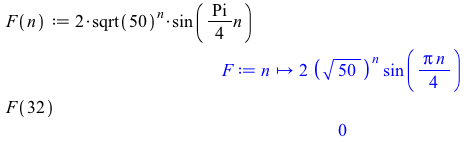
\includegraphics[width=0.75\textwidth]{maple.png}
	\caption{utskrifter från Maple vid beräknings av $x_{32}$}
	\label{fig:maple}
\end{figure}

\begin{figure}[h!]
	\centering
	%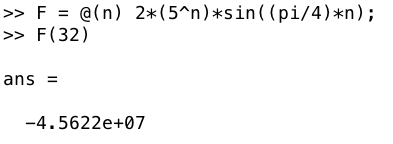
\includegraphics[width=0.75\textwidth]{matlab.png}
	\caption{utskifter från Matlab vid beräknings av $x_{32}$}
	\label{fig:maple}
\end{figure}


\end{document}

